\chapterimage{chapter_head_2.pdf} % Chapter heading image

\chapter{Caraterísticas da dança}

\begin{tcbinformation}{Dança}
\index{Dança}
\label{def:DancaGeral}
Mas que uma simples palavra, a dança é um conceito; e como tal, esta representa 
uma ideia, juízo ou opinião; pelo que podemos ter múltiplas pontos de vista do que é a dança \cite[pp. 2]{Rejane2011}.
%Assim podemos listar os seguintes significados a palavra dança:
\begin{itemize}
\item ``Sequência de movimentos corporais executados de maneira ritmada, 
em geral ao som de música'' \cite[pp. 604]{ferreira1999novo}.
\item ``A arte de mover o corpo segundo a relação estabelecida entre tempo e espaço,
gerada pelo ritmo e a composição coreográfica'' \cite[pp. 17]{bencardinidanca}
\item A dança é a movimentação corporal, que tem como proposito, 
a expressão emocional, sentimental, lúdica ou artística.
%% correr para chegar ao otro lado exersicio, correr paa expresarse dança.
\end{itemize}
\end{tcbinformation} 

\begin{center}
\begin{tabular}{lll}
~ & Sim & Não \\
A dança é sempre feita com música? & \NoCheckedItem & \CheckedItem \\ %\hline
É necessário um par para dançar? & \NoCheckedItem & \CheckedItem \\ %\hline
A dança é uma arte? & \CheckedItem & \NoCheckedItem \\ %\hline
A dança tem necessariamente um significado? & \NoCheckedItem & \CheckedItem \\ %\hline 
%no confundir com: a dança tem um proposito? sim \cite[pp. 10]{schrader2005sense}
\end{tabular}
\end{center}

A primeira afirmação é fácil de entender, pois se neste momento ficamos em pé,
e iniciamos a contar, desde uma perspetiva emocional, a historia de nossa vida, 
utilizando nosso corpo e uma estrutura rítmica escolhida por nós mesmos,
então estaríamos sim dançando; porém sem música de fundo.

Do mesmo exemplo anterior se deduz que não necessitamos um par para nos expressar mediante a dança;
é mais, existem muitas disciplinas da dança em que não se necessita par,
por exemplo o ``free style''.

Seguindo o conceito presentado anteriormente, a dança sim é uma arte \cite[pp. 17]{bencardinidanca}.

A dança não tem que ter necessariamente um significado, 
pois podemos mover-nos ritmicamente pelo simples prazer de fazê-lo, 
sem nenhuma outra pretensão, 
ou também procurando ver o limite de nossas capacidades físicas.

%%%%%%%%%%%%%%%%%%%%%%%%%%%%%%%%%%%%%%%%%%%%%%%%%%%%%%%%%%%%%%%%%%%%%%%%%%%%%%%%

%%%%%%%%%%%%%%%%%%%%%%%%%%%%%%%%%%%%%%%%%%%%%%%%%%%%%%%%%%%%%%%%%%%%%%%%%%%%%%%%
%%%%%%%%%%%%%%%%%%%%%%%%%%%%%%%%%%%%%%%%%%%%%%%%%%%%%%%%%%%%%%%%%%%%%%%%%%%%%%%%
\section{Elementos da dança}
\index{Elementos da dança}
\index{Rudolf Laban}
\begin{wrapfigure}{l}{0.30\textwidth}
\vspace{-10pt}
\centering
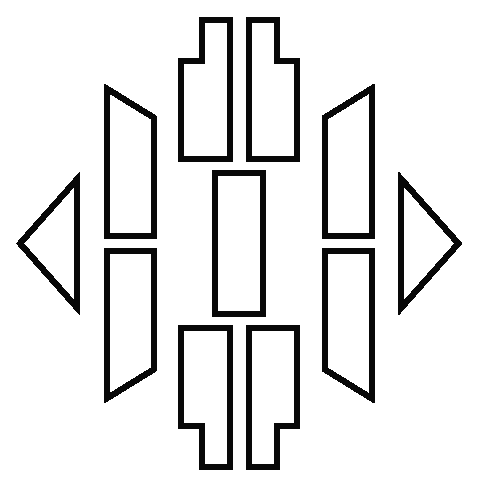
\includegraphics[width=0.28\textwidth]{chapters/cap-dance-elements/Labanotation2.eps}
\caption{Símbolos de Labanotation.}
\label{fig:elementosdanca1old}
\vspace{-10pt}
\end{wrapfigure}
 No seu estudo da teoria do movimento, Rudolf Laban (1879-1958) fez significativas contribuições e
observações na área da ``dança  educacional'',  
realizando contribuições como, a criação de uma forma escrita de notação coreográfica (Labanotation), 
e um  analises preciso do movimento na dança, entre outros \cite[pp. 18]{elementosdanca2017} \cite[pp. 11]{paine2014complete}.

Com seu estudo do movimento, 
Laban  deu sustento ao ensino da dança educativa moderna e 
presentou 16 temas ou áreas-chave no analises do movimento, 
sendo estes ligados a estágios no desenvolvimento das crianças  \cite[pp. 12]{paine2014complete}.

Nas décadas dos anos 1960 e 1970, 
viu-se  na Grã-Bretanha um crescimento importante na dança contemporânea;
a popularidade deste estilo foi devido a que este era menos exclusivo que o balé, 
com técnicas baseadas em movimentos mais naturais, 
além de ter a vantagem de ser unissex e pouco pretensioso.
Assim, estabelecimentos como a ``London School of Contemporary Dance'',
ou bailarinos treinados trabalhando de forma independente,
ofereciam oficinas para faculdades e escolas,
dando um ``enfoque profissional à dança'' \cite[pp. 12]{paine2014complete}.

\begin{wrapfigure}{r}{0.37\textwidth}
\centering
\vspace{-15pt}
%%\smartdiagram[bubble diagram]{Dança, Corpo, Tempo, Espaço, Relações, Dinâmicas}
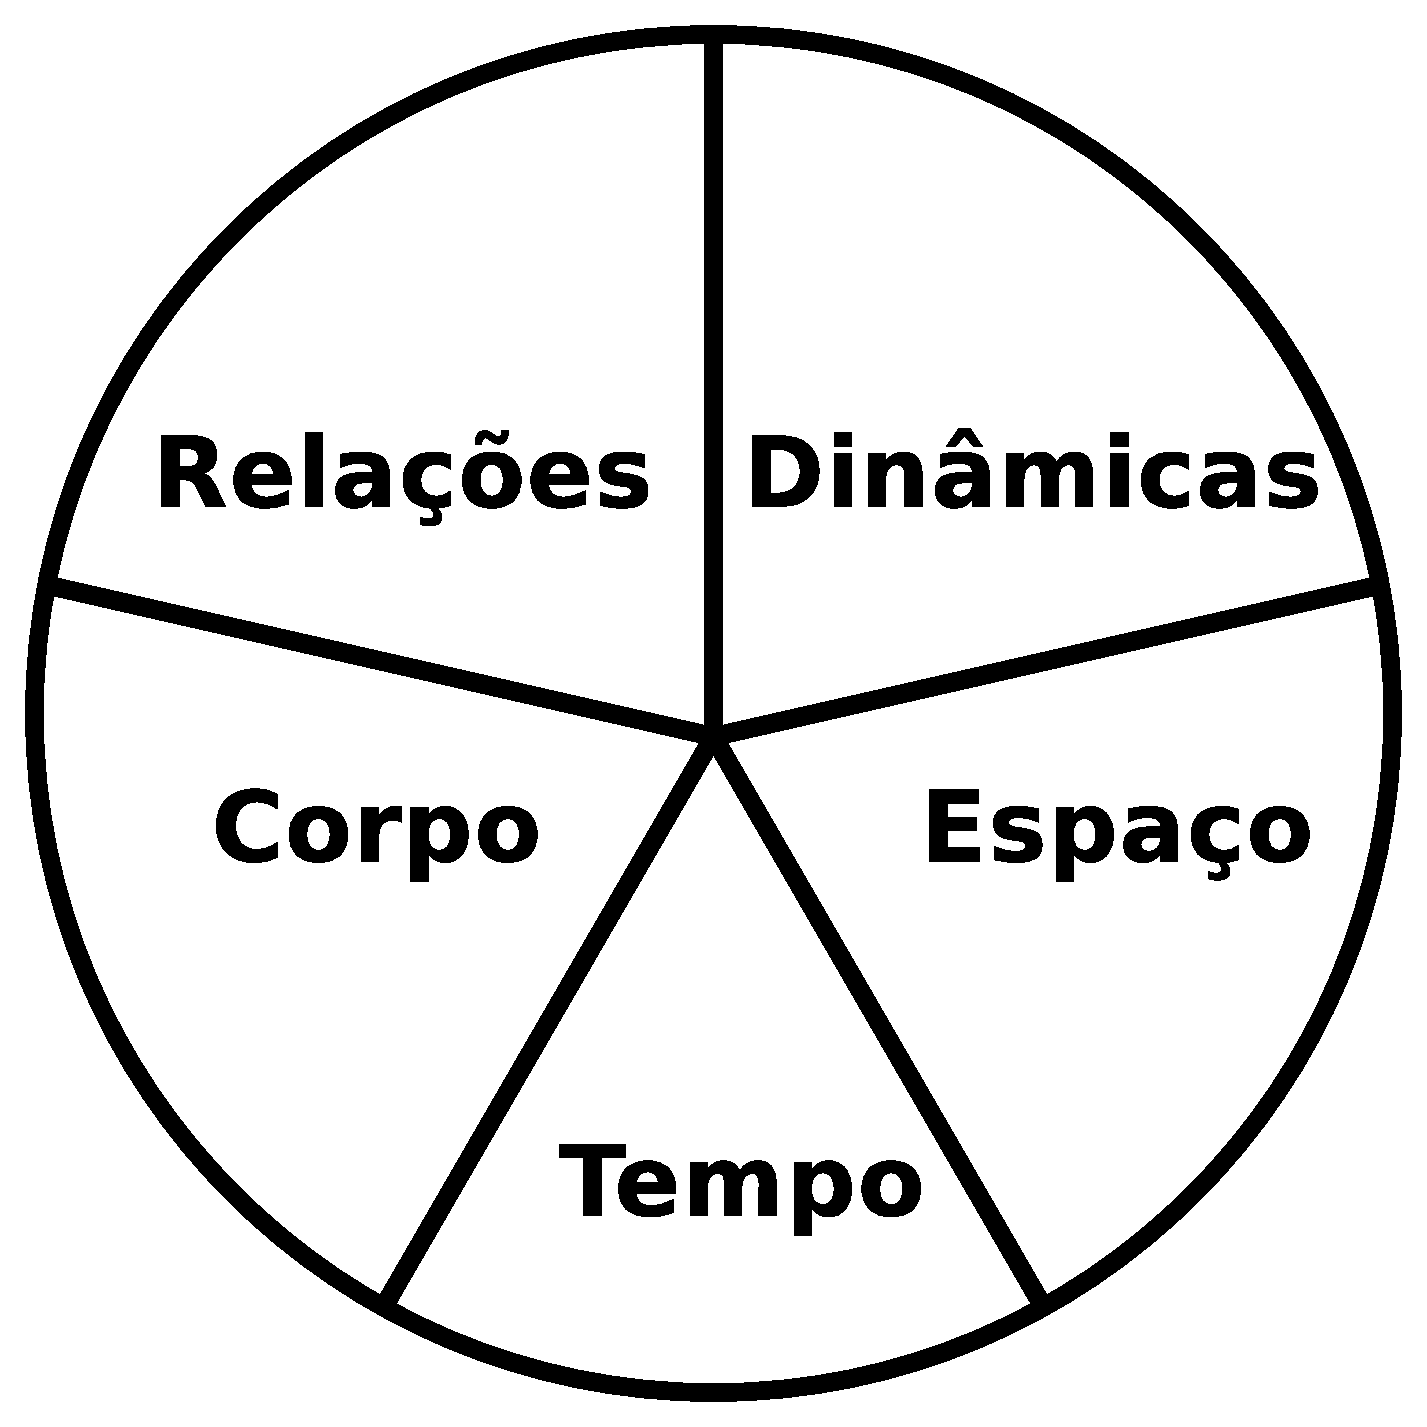
\includegraphics[width=0.35\textwidth]{chapters/cap-dance-elements/DanceElements.eps}
\caption{Elementos da dança}
\label{fig:elementosdanca1}
\vspace{-10pt}
\end{wrapfigure}
Por outro lado, em 1994, Jacqueline Smith-Autard, uma das principais educadoras britânicas de dança, 
propôs um modelo intermediário (``midway model''), entre o educacional e o profissional, 
usando as áreas mais interessantes propostas por Laban \cite[pp. 12]{paine2014complete}.

Seguindo esses modelos, é comum achar na literatura atual 
\cite[pp. 4]{carline2011lesson}       %% corpo, espaço, esforço , relacionamentos
\cite[pp. 13,27]{paine2014complete}   %% corpo, espaço, esforço , relacionamentos
\cite[pp. 69]{schrader2005sense}      %% tempo, espaço, esforço
\cite[pp. 131]{mccutchen2006teaching},%% tempo, corpo, espaço, esforço , relacionamentos
 análises  da dança dividindo esta entre três a cinco elementos,
dependendo da visão do autor.
Estes elementos da dança são: O corpo, as dinâmicas, o espaço, os relacionamentos, e o tempo;
a Figura \ref{fig:elementosdanca1} mostra uma representação gráfica destes elementos.



%%%%%%%%%%%%%%%%%%%%%%%%%%%%%%%%%%%%%%%%%%%%%%%%%%%%%%%%%%%%%%%%%%%%%%%%%%%%%%%%
\subsection{Corpo}
\caracterelement{Do corpo ou das ações}{O que o corpo está fazendo?}
Na dança existem muitos motivos para realizar uma ação corporal;
cada um destes motivos procura ter um significado, seja este prático ou estético, literal ou metafórico \cite[pp. 5]{carline2011lesson}.
As ações realizadas pelo corpo são moldadas pelas relações com os outros elementos da dança,
como as dinâmicas, o uso do espaço, o tempo, e as relações com os outros \cite[pp. 5]{carline2011lesson}.
Algumas das ações mais básicas que podemos realizar com o corpo são,
desloca-nos, pular, virar-nos, gesticular, ou quietude \cite[pp. 27]{paine2014complete}.

\textbf{Deslocamentos:} Implica a transferência do peso do corpo 
para variar de posição no espaço usando na dança;
existem várias formas de realizar esta ação,
por exemplo podemos faze-o pisando, deslizando, rastejando \cite[pp. 28]{paine2014complete}.

\textbf{Pular:} (ou elevar-nos) descreve a ações que provocam que o corpo saia e volta ao chão,
impulsando-nos pelo uso das pernas; as distancias alcançadas podem ser pequenas ou longas,
dependendo do método que usemos no movimento  \cite[pp. 28]{paine2014complete}. 

\textbf{Virar:} envolve movimentos de rotação em torno de um eixo.
Este giro não tem que ser necessariamente completo ($360^o$),
e podem ser trabalhados níveis, como giros de um ângulo especifico;
os movimentos de giro podem ser iniciados por alguma parte do corpo, 
não necessariamente pelos pés \cite[pp. 29]{paine2014complete}.

\textbf{Gesto:} Implica o movimento de uma ou varias partes do corpo,
que não envolve suporte ou transferência de peso
(ex: movimentos axiais, como flexão, alongamento e torção);
os gestos enriquecem o conteúdo expressivo de uma dança,
onde são usados para contar uma história, 
usando um vocabulário simbólico reconhecido popular ou tradicionalmente 
\cite[pp. 29]{paine2014complete}.

\textbf{Quietude:} descreve a capacidade de interromper nosso movimento, 
controlando no processo nosso equilíbrio \cite[pp. 29]{paine2014complete}.


A consciência corporal se centra no estudo do uso controlado do corpo, 
à medida que as movimentações são exploradas,
já sejam  estes movimentos realizados pelo corpo inteiro,
ou por partes isoladas deste \cite[pp. 5]{carline2011lesson}.
O tema da consciência corporal será abordado com maior aplitude  na Seção \ref{sec:BodyAwareness}.


%%%%%%%%%%%%%%%%%%%%%%%%%%%%%%%%%%%%%%%%%%%%%%%%%%%%%%%%%%%%%%%%%%%%%%%%%%%%%%%%
\subsection{Dinâmica (esforço)}
\caracterelement{Das dinâmicas}{Como o corpo está se movendo?}
As dinâmicas no movimento 
indicam o jeito em que a energia será usada e direcionada no corpo durante a dança \cite[pp. 131, 136]{mccutchen2006teaching};
além de provocar em nossos movimentos algo que poderia ser definido, metaforicamente, como textura ou cor;
dando uma identidade própria a cada movimento, dependendo da dinâmica utilizada;
por exemplo, não é o mesmo dar um passo de forma lenta como tentando não fazer barulho,
que dar o passo caindo como se estivéssemos bêbados.

Rudolf Laban, no seu estudo do movimento, 
dividiu as dinâmicas (ou ``esforço'' na notação de Laban) 
em quatro categorias ou fatores: peso, tempo, espaço e fluxo 
\cite[pp. 5]{carline2011lesson}
\cite[pp. 30]{paine2014complete}.
Porem, o modelo de Laban não é a única forma em que podemos fatorar as dinâmicas,
de modo que, inclusive a escolha do modelo para descrever as dinâmicas,
influencia na textura percebida na realização do movimento \cite[pp. 30]{paine2014complete}. 

Uma explicação detalhada, dos fatores nos quais podemos dividir as 
\hyperref[subsec:fatordinamica]{\textbf{dinâmicas do movimento}},
pode ser encontrada na Seção \ref{subsec:fatordinamica};
com este propósito serão mostrados diferentes modelos propostos por vários autores,
sobre como podem ser fatoradas as dinâmicas.



%%%%%%%%%%%%%%%%%%%%%%%%%%%%%%%%%%%%%%%%%%%%%%%%%%%%%%%%%%%%%%%%%%%%%%%%%%%%%%%%
\subsection{Espaço} 
\caracterelement{Do espaço}{Para onde o corpo se está movendo?}
A maneira como o espaço é usado pode ajudar a dar interesse visual a nossa dança,
ajudando-nos a contar uma historia como nosso corpo, com um relato que progride no tempo 
\cite[pp. 6]{carline2011lesson}
\cite[pp. 31]{paine2014complete}
\cite[pp. 131, 136]{mccutchen2006teaching}; 
alguns aspectos do espaço que podem ser interessantes de ser explorados na nossa dança são:

\textbf{Espaço pessoal e geral:}  Trabalhamos no nosso espaço pessoal 
quando realizamos movimentos sem deslocamento 
(ex: tremer, subir, girar, pausar ou afundar);
e em nosso espaço geral quando nos deslocamos a outras posições
(ex: caminhar, correr, pular) \cite[pp. 7]{carline2011lesson}
\cite[pp. 32]{paine2014complete}.

\textbf{Caminhos:} Podemos definir o caminho como o padrão desenhado no chão ou no ar, 
quando nos deslocamos,
esta padrão pode ser uma única linha reta ou 
varias conectadas formando padrões mais complexos, 
 com zigue-zagues; também poderíamos ter caminhos curvos e sinuosos; 
inclusive o caminho pode ser uma curva sem inicio né fim como um círculo 
\cite[pp. 7]{carline2011lesson}
\cite[pp. 32]{paine2014complete}.



\textbf{Direções:} Quando trabalhamos com direções, 
temos a possibilidade que nosso movimento seja 
para frente, para trás, para os lados, para cima, para baixo, em diagonal,
entre outras 
\cite[pp. 7]{carline2011lesson}
\cite[pp. 32]{paine2014complete}
\cite[pp. 97-98]{schrader2005sense}. 


\textbf{Formas do corpo:} Com nosso corpo, ou grupo de corpos, podemos criar formas diferentes,
como emular uma parede, uma esfera, 
ou podemos fazer posturas mediante torções, 
e movimentando de forma independente distintas partes do corpo 
\cite[pp. 8]{carline2011lesson}
\cite[pp. 32]{paine2014complete}
\cite[pp. 97]{schrader2005sense}.

\textbf{Níveis:} Quando usamos nosso corpo, 
podemos quantificar nossos movimentos em vários níveis,
relacionados com a distancia com o chão;
por exemplo ao pular, este movimento pode ser baixo, meio ou alto 
\cite[pp. 8]{carline2011lesson}
\cite[pp. 32]{paine2014complete}
\cite[pp. 96]{schrader2005sense}.

\textbf{Posição e proximidade:}  (Preposições espaciais)
É possível usar preposições que nos ajudem a descrever, o uso do espaço,
em relação à posição e proximidade; entre os termos que podemos usar temos:
atrás, na frente, 
acima, abaixo, 
perto, longe, 
através, ao redor
\cite[pp. 32]{paine2014complete} 
\cite[pp. 9]{carline2011lesson}, etc.

\textbf{Dimensão} (Tamanho do movimento ou forma) 
Indica a dimensão de grandeza ou amplitude que terá o movimento ou a forma que executemos;
assim, podemos escolher valores de dimensão entre pequeno e grande 
\cite[pp. 32]{paine2014complete} 
\cite[pp. 99]{schrader2005sense}.

%\textbf{Bases do corpo:}  \cite[pp. 8]{carline2011lesson}.

%\textbf{Extensões para o espaço:}  \cite[pp. 9]{carline2011lesson}.

%%%%%%%%%%%%%%%%%%%%%%%%%%%%%%%%%%%%%%%%%%%%%%%%%%%%%%%%%%%%%%%%%%%%%%%%%%%%%%%%
\subsection{Relacionamento} 
\caracterelement{Das relações}{Com quem ou com que o corpo está se movendo?}
Na dança podemos nos movimentar relacionando-nos com outra pessoa, como na dança social a  dois,
ou em grupos, como em algumas danças folclóricas.
Quando dançamos podemos liderar a dança ou ser seguidores, 
também podemos nos deslocar indo ao encontro com o grupo, 
ou nos separar, dividir, espelhar, contrastar, 
estar em cânone, em uníssono, ou alguma outra forma;
a forma de nos relacionar com os demais são variadas,
inclusive podemos interagir como objetos, sejam estes reais ou imaginários
 \cite[pp. 9]{carline2011lesson}
 \cite[pp. 27, 32-33]{paine2014complete}
\cite[pp. 131, 132, 134]{mccutchen2006teaching}.


%%%%%%%%%%%%%%%%%%%%%%%%%%%%%%%%%%%%%%%%%%%%%%%%%%%%%%%%%%%%%%%%%%%%%%%%%%%%%%%%
\subsection{Tempo}
\caracterelement{Do tempo nas ações}{Quando o corpo realiza uma ação?}
O movimento e as pausas que realizamos estão sempre ligados à variável tempo,
tendo estes um tempo inicial e uma duração;
assim, nossos movimentos, vistos de forma sequencial no tempo, 
seguem um ritmo que pode ser marcado livremente por nós,
ou pode tentar seguir uma fonte externa de informação, como a música;
em qualquer caso o dançarino é o encarregado desta escolha criativa;
existem alguns termos que devem ser parte de nosso vocabulário de dança,
quando estudamos o aproveitamento do elemento tempo,
estes são: 
\hyperref[ref:Pulso]{\textbf{pulso}}, 
\hyperref[sec:Tempo]{\textbf{tempo}}, 
\hyperref[sec:Andamento]{\textbf{andamento}}, 
\hyperref[sec:pos:Ritmo]{\textbf{ritmo}}, e 
\hyperref[def:Metrica]{\textbf{métrica}}
\cite[pp. 82]{schrader2005sense}
\cite[pp. 131, 134, 136]{mccutchen2006teaching}.

%%%%%%%%%%%%%%%%%%%%%%%%%%%%%%%%%%%%%%%%%%%%%%%%%%%%%%%%%%%%%%%%%%%%%%%%%%%%%%%
% FALTA INCLUIR ENERGIA
%%%%%%%%%%%%%%%%%%%%%%%%%%%%%%%%%%%%%%%%%%%%%%%%%%%%%%%%%%%%%%%%%%%%%%%%%%%%%%%
%% https://books.google.com.br/books?id=C0yjXGJ3EEoC&pg=PA131&dq=dynamics+dance+energy&hl=pt-BR&sa=X&ved=0ahUKEwjc472wjrXlAhUeEbkGHbstBbUQ6AEIKTAA#v=onepage&q=dynamics%20%20energy&f=false
%% https://books.google.com.br/books?id=omYS0_FkOWIC&pg=PT169&dq=dynamics+dance+energy&hl=pt-BR&sa=X&ved=0ahUKEwjc472wjrXlAhUeEbkGHbstBbUQ6AEIMjAB#v=onepage&q=dynamics%20energy&f=false
%% https://books.google.com.br/books?id=Z0hoAwAAQBAJ&printsec=frontcover&dq=discovering+dance&hl=pt-BR&sa=X&ved=0ahUKEwif04WJwbXlAhUkILkGHdxnAjEQ6AEIKTAA#v=onepage&q=discovering%20dance&f=false
%%%%%%%%%%%%%%%%%%%%%%%%%%%%%%%%%%%%%%%%%%%%%%%%%%%%%%%%%%%%%%%%%%%%%%%%%%%%%%%
%%%%%%%%%%%%%%%%%%%%%%%%%%%%%%%%%%%%%%%%%%%%%%%%%%%%%%%%%%%%%%%%%%%%%%%%%%%%%%%

%%%%%%%%%%%%%%%%%%%%%%%%%%%%%%%%%%%%%%%%%%%%%%%%%%%%%%%%%%%%%%%%%%%%%%%%%%%%%%%%

\section{Decorando passos de dança}
\label{sec:decorando-passos-de-danca}
Os professores de dança Aurélio e Neiliane,
mediante sua ``Escola de Dança on-line'' e seu projeto 
\href{https://www.facebook.com/dancandoeaprendendo/}{Dançando e Aprendendo}, 
entre outras muitas dicas de dança,
propõem
a utilização de uma \href{https://www.youtube.com/watch?v=ePwjQx5egAo}{``folha de memorização de passos''} 
para melhorar o aprendizado de passos de dança 
e a retenção destes na \hyperref[sec:memoria:longo]{\textbf{memória de longo prazo}}.

A proposta consiste em preencher uma destas folhas de memorização
por cada passo aprendido (ou em processo de aprender),
de modo que nela primeiro devemos colocar um título ou um nome de passo,
isto como um recurso mnemotécnico e para ajudar-nos a catalogar o passo em nosso acervo pessoal.
A folha também pede ao usuário uma descrição verbal do passo com luxo de detalhes, 
colocando estas informações como se fossem escritas para ser lidas por uma pessoa 
que não assistiu à aula onde ensinaram o passo; 
sendo esta uma forma em que você do presente pode enviar 
uma mensagem digerível e estruturada a você do futuro
sobre a mecânica de um passo de dança.
Outro item que pede a folha é agregar algum comentário que por associação 
te faça lembrar o movimento; por exemplo, no passo ``Romário'' se poderia anotar que 
o movimento é chamado assim porque se dá um chute, ou 
no movimento ``Puladinho'' pode-se anotar que este nome vem da frase ``para o ladinho'' pois no passo 
se vá para um lado e logo para outro.
Finalmente a folha recomenda ao usuário
ensinar o passo aprendido a um amigo imaginário,
com o fim de garantir que as informações antes escritas estejam completas 
e sejam coerentes.

\begin{tcbattention}
Na Pag. \pageref{pos:page:folhamemorizacao} 
podemos ver uma forma compacta da folha de memorização 
de passos proposta pelos professores Aurélio e Neiliane; porém,
recomendo fortemente ir ao 
\href{https://www.youtube.com/watch?v=ePwjQx5egAo}{sitio web}
dos professores para ver a forma extendida desta folha.
\end{tcbattention}

Além de todas estas indicações, 
propostas pelos professores Aurélio e Neiliane
na folha de memorização,
só agregaria que também deveriam ser anotadas referencias 
à data, o lugar e ao professor; pois um recurso como esta folha é muito importante
para contribuir com a documentação dos diferentes estilos, didáticas e informações
que podem ser achados na dança de salão no Brasil;
por exemplo, com o tempo uma pessoa poderia considerar que o conhecimento 
acumulado no seu acervo pode formar um livro, 
e este já estaria bem documentado e referenciado.

A folha de memorização de passos também atinge um ponto 
que foi a motivação principal para escrever este livro;
sendo esta, a necessidade de ter um método de notação coreográfica que permita, 
mediante símbolos e/ou texto, representar e descrever os movimentos executados
nos passos no samba de gafieira. Assim, 
a só existência da folha de memorização de passos, fomenta a ativação da 
inteligencia coletiva das pessoas que estão no mundo da dança 
a procurar ou criar algumas formas de notação coreográfica que permitam 
plasmar toda esta informação em palavra escrita.


 



\newpage
\thispagestyle{plain}
\begin{center}\TITULOA{Folha de memorização de passos}\end{center}
\label{pos:page:folhamemorizacao}

\begin{center}\Large\textit{ Esta folha é uma ferramenta simples de memorização e registro dos passos aprendidos.}\end{center}

\TITULOB{Nome do passo aprendido}
\noindent Digite no espaço o nome do passo que você aprendeu.

\BOXDATA\;

\TITULOB{Passo a passo} 
\noindent Descreva abaixo (com riqueza de detalhes) todo o passo a passo da
figura que você aprendeu. Descreva cada ação feita para realizar o passo.
É importante que sua anotação seja possível de ser entendida por outra 
pessoa além de você, portanto não economize nos detalhes do passo.

\LINEDATA\;
\LINEDATA\;
\LINEDATA\;
\LINEDATA\;
\LINEDATA

\TITULOB{Suas conexões}	
\noindent Escreva aqui que conexões (imagens cotidianas, histórias etc.)
você pode fazer para te ajudar a lembrar do passo que você acabou de aprender.
O que é presente no seu cotidiano que se você fizesse uma associação ao passo
te ajudaria a lembrar dele?

\LINEDATA\;
\LINEDATA\;
\LINEDATA

\TITULOB{Ensine ao amigo imaginário}
\noindent Para fechar o processo de aprendizado, ensine o passo que você aprendeu.
O ato de ensinar não só reforça o seu aprendizado como também te ajuda a
compreensão do passo, haja vista que para ensinar é necessário domínio do
que está sendo ensinado. Portanto, ensine o passo aprendido para o amigo 
imaginário.\\

\FOOTPAGE\;


%%%%%%%%%%%%%%%%%%%%%%%%%%%%%%%%%%%%%%%%%%%%%%%%%%%%%%%%%%%%%%%%%%%%%%%%%%%%%%%%
\section{Rota de estudo na danca de salão}
\label{sec:dance-elements-processo}
Nesta seção é presentada uma proposta de rota de estudo para o aprendizado da
dança de salão. 
Como mostra a Figura \ref{fig:dance-elements-processo},
a proposta está basejada em 3 níveis de trabalho.
\begin{figure}[!h]
\centering
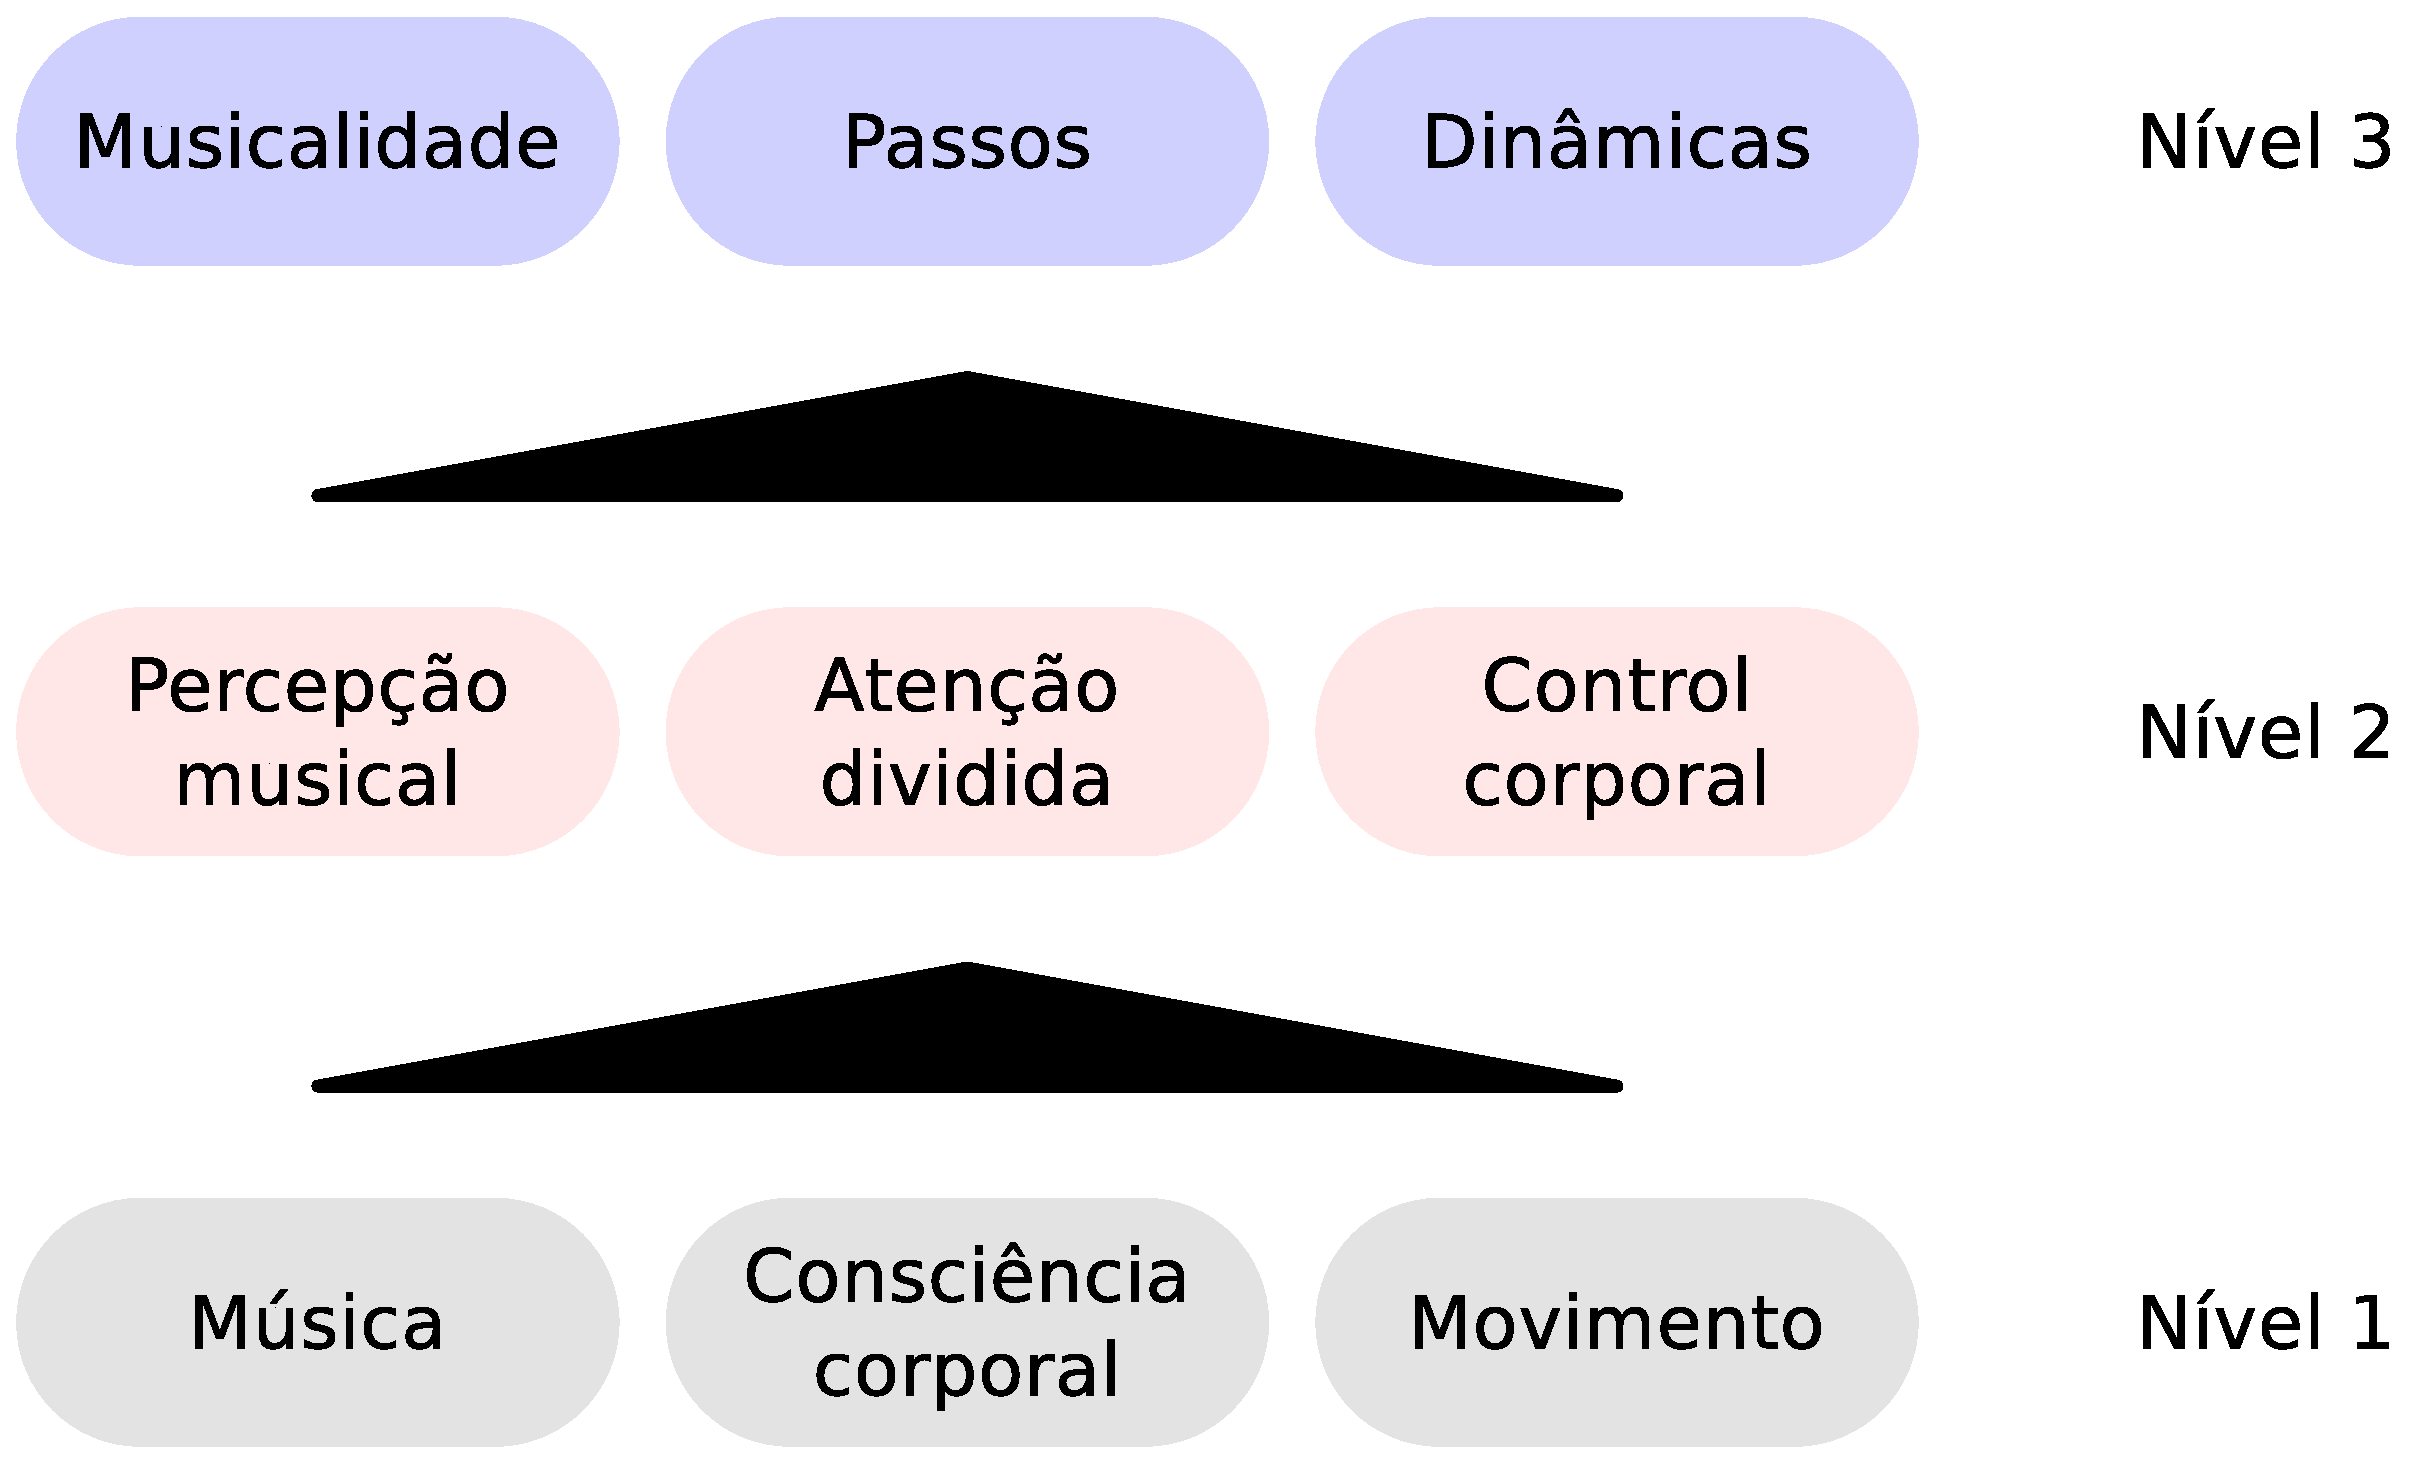
\includegraphics[width=0.7\textwidth]{chapters/cap-dance-elements/Diagrama-danca.eps}
\caption{Rota de estudo para o aprendizado da dança de salão.}
\label{fig:dance-elements-processo}
\end{figure}
\begin{itemize}
\item No nível 1 temos os temas mais básicos a serem estudados quando
iniciamos nosso percorrido na dança, estes são:
A teoria musical, a qual pode ser vista nos 
Capitulos \ref{cap:musicabasica}, \ref{cap:musicacomposer} e \ref{cap:musicatopicos}.
A consciência corporal, que é estudada no Capítulo \ref{fig:bodyrelations}.
O movimento, que corresponde ao aprimoramento de nossa aptidão física.
\item No nível 2 se inicia o perfeicionamento de habilidades,
mediante a combinação de vários componentes aprendidos no nível 1, estes são:
A percepção musical, a qual pode ser vista no Capítulo \ref{cap:percepcaomusical}.
O controle corporal, que é estudada no Capítulo \ref{fig:bodyrelations}.
A atenção dividida, que é estudada nos Capítulos \ref{cap:aprendizagem} e \ref{chap:trainingbodycontrol}.
\item No nível 3 são listados os temas mais complexos os quais
requerem conhecimentos do nível 1 e/ou 2 para serem satisfatoriamente completados,
estes são:
A musicalidade, a qual pode ser vista nos Capítulos \ref{chap:FundamentosMusicalidade} e \ref{chap:TopicosMusicalidade}.
As dinâmicas nos movimentos, que são estudadas na Seção \ref{sec:musicalidade:dinamicas}.
Os passos de dança, que são listados no Capítulo \ref{chap:passos-samba-gafieira}.
\end{itemize}
A proposta de estudo da Figura \ref{fig:dance-elements-processo} não aponta a que 
todo mundo deva inciar do nível 1, 
pois dependendo da experiencia de vida de cada pessoa estas podem ter conhecimento de itens
em vários níveis no momento de iniciar seu aprendizado na dança de salão.
A proposta presentada busca dar uma direção ao fluxo de estudos de um entusiasta à dança de salão.


